\documentclass[12pt,a4paper,onecolumn]{article}

% Encoding and language
\usepackage[utf8]{inputenc}
\usepackage[T1]{fontenc}
\usepackage[english]{babel}

% Font
\usepackage{times}
\usepackage[normalem]{ulem}

% Set margins
\usepackage[a4paper, top=2cm, bottom=2cm, left=2.5cm, right=2.5cm]{geometry}

% Tabulation
\usepackage{tabto}

% Line spacing
\usepackage{setspace}
\onehalfspacing

% Page numbers
\usepackage{fancyhdr}
\pagestyle{fancy}
\fancyhf{} % Clear default header/footer
\rfoot{\thepage} % Right-aligned page numbers in footer

% Remove page number from cover/abstract/etc
\usepackage{titlesec}
\newcommand{\noPageNumber}{\thispagestyle{empty}}

% Prevent indentation
\setlength{\parindent}{0pt}
\setlength{\parskip}{0.5em}

% Table
\usepackage{booktabs}

% Figure management
\usepackage{graphicx}
\usepackage{caption}
\usepackage{subcaption}
\usepackage{wrapfig}

\usepackage{pgfplots}
\pgfplotsset{compat=1.16}
\def\mathdefault#1{#1}
\everymath=\expandafter{\the\everymath\displaystyle}

% Subfigure management
\usepackage{layouts}
%\usepackage{floatrow}
%\usepackage[label font=bf,labelformat=simple]{subfig}% <-- changed
%\floatsetup[figure]{style=plain,subcapbesideposition=top}


% Optional: headings formatting
\titleformat{\section}{\large\bfseries}{\thesection}{1em}{}
\titleformat{\subsection}{\normalsize\bfseries}{\thesubsection}{1em}{}

% Optional: remove widow/orphan lines
\widowpenalty=10000
\clubpenalty=10000

% Mathematics
\usepackage{amsmath,mathtools,amssymb} 

% References
\usepackage[backend=biber, style=authoryear]{biblatex}
\addbibresource{Bibliography.bib}
\DeclareBibliographyCategory{main}
 \nocite{*}
\addbibresource{Survey.bib}
\DeclareBibliographyCategory{survey}
 \nocite{*}

\begin{document}
 %% textwidth in cm: \printinunitsof{in}\prntlen{\textwidth}

\begin{titlepage}
   \begin{center}
      
\includegraphics[width=0.65\textwidth]{logos.png}
      

       \textbf{\Huge Gap year Internship Report}

       \vspace{0.5cm}
       \LARGE Evaluating the impact of maturation time variability in stage-structured host-parasitoid models.
            
       \vspace{1cm}

       \textbf{Mathis Drieu}

        \vspace{1cm}
        \normalsize
        Under the supervision of\\
        Quentin Guilloit, Jules Guilberteau, Thierry Spataro
        \vspace{0.5cm}

        
        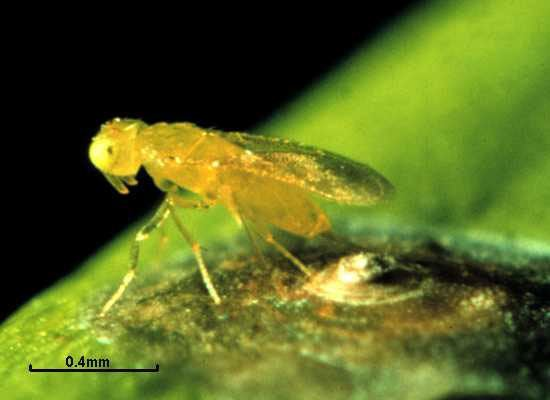
\includegraphics[width=0.70\textwidth]{aphytis-melinus.jpeg}
        \small\textnormal\\
        Parasitoid \textit{Aphytis melinus} and its host \textit{Aonidiella aurantii}, a pest of citrus in California and elsewhere (Alchetron encyclopedia).
       
       
       \vspace{0.5cm}
        \large   
       IEES, Sorbonne Université\\
       Team DYNECO\\
       \normalsize February-June 2025\\
       
            
   \end{center}
\end{titlepage}

\newpage


Lou pue

\end{document}